\documentclass[7.5pt,a4paper, landscape]{article}
\usepackage{amsmath, amssymb, amsthm}
\usepackage[
    % total={130mm,277mm},
    % a4paper,
    top=0mm,
    bottom=1mm,
    left=1mm,
    % right=2mm,
    marginparwidth=1mm,
    marginparsep=0mm,
    centering]{geometry}
\usepackage{multicol}
\usepackage{booktabs}
\usepackage{graphicx} 
\setlength{\columnsep}{8pt}
\setlength{\parindent}{0pt}
\setlength{\parskip}{0pt}
\usepackage{enumitem}
\setlist{noitemsep,topsep=1pt,parsep=1pt,partopsep=0pt}
\setlist[itemize]{leftmargin=*}

% \setlength{\fboxsep}{3pt} % Reduce inner padding
\setlength{\fboxrule}{0.1pt} % Reduce border thickness

\renewcommand{\baselinestretch}{1.2}

\begin{document}

\scriptsize

\begin{multicols*}{4} % Use multicols* environment for better column balancing

\fbox{\begin{minipage}[t]{\linewidth}
\textbf{Realizable (Separable) case}
When there is a model that separates perfectly.
There is \( h^* \in \mathcal{H} \) that achieves perfect separation between classes, i.e. zero true loss:  
    $ L_({\mathcal{D},f})(h^*) = 0$, in-sample loss \( L_S(h^*) = 0 \)

\textbf{Agnostic case}
    When there is no perfect separator, find the best imperfect one
\end{minipage}}

% \vspace{\baselineskip} % Add vertical space between boxes

\fbox{\begin{minipage}[t]{\linewidth}
\textbf{Empirical loss/risk }
of any hypothesis \( h \in H \) as
$ L_S(h) \overset{\text{def}}{=} \frac{|\{i \in [m] : h(x_i) \neq y_i\}|}{m}$
\end{minipage}}

% \vspace{\baselineskip}

\fbox{\begin{minipage}[t]{\linewidth}
\textbf{Assumption (iid):} Examples are independent and identically distributed according to $\mathcal{D}$ ($S \sim \mathcal{D}^m$)
\textbf{ERM Algorithm A:} Check all $h \in \mathcal{H}$
, Pick $h_S = \operatorname*{argmin}_{h \in \mathcal{H}} L_S(h)$. 
This $h_S$ is the best we can do with the data, but may not be perfect on unseen data
\end{minipage}}

% \vspace{\baselineskip}

\fbox{\begin{minipage}[t]{\linewidth}
\textbf{Sampling Bound in Realizable Finite Case}
With assumptions of realizability and finite $\mathcal{H}$:
\[ m \geq \frac{\log(|\mathcal{H}|/\delta)}{\epsilon} \]
suffices for $\epsilon$, $\delta$ guarantee:
\[ \mathbb{P}[L_{D,f}(h_S) \leq \epsilon] \geq 1 - \delta \]
\end{minipage}}

% \vspace{\baselineskip}

\fbox{\begin{minipage}[t]{\linewidth}
For $0 < p < 1$: $(1 - p)^{\frac{1}{p}} \leq \frac{1}{e}$

$ P(A \cup B) \leq P(A) + P(B) $

Accuracy parameter, $\epsilon$: how far output classifier can be from the optimal one. 

Confidence parameter,$1- \delta$: Probability of getting a non-representative sample
\end{minipage}}

% \vspace{\baselineskip}

\fbox{\begin{minipage}[t]{\linewidth}
\textbf{PAC Learnability}
\\ A hypothesis class $\mathcal{H}$ is PAC learnable if:
\begin{itemize}
    \item There exists a function $m_{\mathcal{H}}:(0,1)^2 \to \mathbb{N}$
    \item And an algorithm that for every $\epsilon, \delta$, distribution $D$ over $X$:
    \begin{itemize}
        \item With realizability assumption
        \item On $m \geq m_{\mathcal{H}}(\epsilon, \delta)$ i.i.d samples from $D$
        \item Finds $h$ satisfying $L(D,f)(h) \leq \epsilon$
        \item With probability $\geq 1 - \delta$
    \end{itemize}
\end{itemize}

\textbf{Corollary} Every finite hypothesis class is PAC learnable with sample complexity
$m_{\mathcal{H}}(\epsilon, \delta) \leq \left\lceil \frac{\log(|\mathcal{H}|/\delta)}{\epsilon} \right\rceil.$ 
Min. integer that satisfies the requirement of PAC learning
\end{minipage}}

% \vspace{\baselineskip}

\fbox{\begin{minipage}[t]{\linewidth}
\textbf{Agnostic PAC Learnability}
\begin{itemize}
    \item Modified data generating distribution: $D$ over $X \times Y$
    \item True risk: \\ $L_D(h) \overset{\text{def}}{=} \mathbb{P}_{(x,y) \sim D}[h(x) \neq y]$
    \item Finds $h$ satisfying \\ $L_D(h) \leq \min_{h' \in \mathcal{H}} L_D(h') + \epsilon$
    \item With probability $\geq 1 - \delta$
\end{itemize}
vs PAC learning: Learner is required to achieve a small error in absolute terms, not relative to best error achievable by hypothesis class
\end{minipage}}

% \vspace{\baselineskip}

\fbox{\begin{minipage}[t]{\linewidth}
\textbf{Generalized Loss}
\begin{itemize}
    \item Domain $Z$, loss function $\ell: \mathcal{H} \times Z \rightarrow \mathbb{R}_+$
    \item True risk (expected loss of a classifier $ h \in \mathcal{H}$, wrt a probability distribution $D$ over $Z$, objects $z$ picked randomly according to $D$): \\ $L_D(h) = \mathbb{E}_{z \sim D}[\ell(h, z)]$
    \item Empirical risk (expected risk over a given sample $S = (z_1,..z_m)$): \\ $L_S(h) = \frac{1}{m} \sum_{i=1}^m \ell(h, z_i)$
\end{itemize}
\end{minipage}}

% \vspace{\baselineskip}

\fbox{\begin{minipage}[t]{\linewidth}
\textbf{Representative Samples}
% \\(To find a $h$ that does well outside training data)
\\ $S$ is $\epsilon$-representative w.r.t $(Z, \mathcal{H}, D)$ if:
\\ $ \forall h \in \mathcal{H}, |L_S(h) - L_D(h)| \leq \epsilon $
($S$ gives good est. of the true loss for each $h$)
\\ Notion of representativeness independent of $H$ and $Z$: 
\textbf{Lemma}
If $S$ is $\frac{\epsilon}{2}$-representative, and $h_S \in \operatorname*{argmin}_{h\in\mathcal{H}} L_S(h)$, then
    $L_{\mathcal{D}}(h_S) \leq \min_{h'\in\mathcal{H}} L_{\mathcal{D}}(h') + \epsilon$

With representative data, the best empirical trained mode $h_s$ is almost as good as best model for $D$. \\
\\
Proof: 
\noindent For every $h \in \mathcal{H}$:
\[
L_{\mathcal{D}}(h_S) \leq L_S(h_S) + \tfrac{\epsilon}{2} 
\leq L_S(h) + \tfrac{\epsilon}{2} 
\leq L_{\mathcal{D}}(h) + \epsilon
\]
\end{minipage}}


\fbox{\begin{minipage}[t]{\linewidth}
    \textbf{Uniform Convergence} \\ $\mathcal{H}$ has uniform convergence if there is function $m_{\mathcal{H}}^{UC}: (0,1)^2 \to \mathbb{N}$ (minimal sample complexity of obtaining UC property)
    \begin{itemize}
        \item Such that a random sample $S \sim \mathcal{D}^m$ of size $m \geq m_{\mathcal{H}}^{UC}(\epsilon, \delta)$
        \item Is $\epsilon$-representative with probability at least $1 - \delta$
    \end{itemize}
    
    \textbf{Corollary}
    If $\mathcal{H}$ has uniform convergence with $m_{\mathcal{H}}^{UC}$, then $\mathcal{H}$ is agnostically PAC learnable with 
    $m_{\mathcal{H}}(\epsilon, \delta) \leq m_{\mathcal{H}}^{UC}\left(\frac{\epsilon}{2}, \delta\right) $. 
    
    \textbf{Theorem}
    \begin{itemize}

    \item Every finite $\mathcal{H}$ has uniform convergence
        i.e. Given a random $S$ of suitable size $m \geq m_{\mathcal{H}}^{UC}\left(\frac{\epsilon}{2}, \delta\right) $,  
        $ \mathbb{P}[\exists h \in \mathcal{H}: |L_S(h) - L_D(h)| > \epsilon] \leq \delta $
    \item And therefore every finite $\mathcal{H}$ is agnostic PAC-learnable
    \item Proof: Using Chernoff-Hoeffding bound
    \end{itemize}
\end{minipage}}


\fbox{\begin{minipage}[t]{\linewidth}
\textbf{Chernoff-Hoeffding Bound} \\
By the law of large numbers, states that when $m$ goes to infinity, empirical averages converge to their true expectation. \\
For random variables $\theta_i$ ($\theta_i = \ell(h, z_i)$) with average $\frac{1}{m}\sum_{i=1}^m \theta_i = L_S(h)$ and expected value $\mu = L_D(h)$:
% Law of large numbers: with increasing $m$, 
\[ P\left[\left|\frac{1}{m}\sum_{i=1}^m \theta_i - \mu\right| > \epsilon\right] \leq 2e^{-2m\epsilon^2} \]

Choose $m \geq \frac{\log(2|\mathcal{H}|/\delta)}{2\epsilon^2} $
\end{minipage}}



\fbox{\begin{minipage}[t]{\linewidth}
\textbf{Corollary}
Let \( \mathcal{H} \) be a finite hypothesis class, let \( Z \) be a domain, and let \( \ell : \mathcal{H} \times Z \to [0,1] \) be a loss function. Then, \( \mathcal{H} \) enjoys the uniform convergence property with sample complexity

\[m_{\mathcal{H}}^{UC}(\epsilon, \delta) \leq \left\lceil \frac{\log(2|\mathcal{H}|/\delta)}{2\epsilon^2} \right\rceil.\]

Furthermore, the class is agnostically PAC learnable using the ERM algorithm with sample complexity

$m_{\mathcal{H}}(\epsilon, \delta) \leq m_{\mathcal{H}}^{UC}(\epsilon/2, \delta) \leq \left\lceil \frac{2\log(2|\mathcal{H}|/\delta)}{\epsilon^2} \right\rceil.$
\end{minipage}}



\fbox{\begin{minipage}[t]{\linewidth}
\textbf{Proof}
Fix some $\epsilon, \delta$. We need to find a sample size $m$ that guarantees that for any $D$, with probability of at least $1 - \delta$ of the choice of $S = (z_1, \ldots, z_m)$ sampled
i.i.d. from $D$ we have that for all $h \in \mathcal{H}$, $|L_S(h) - L_D(h)| \leq \epsilon$. That is,

\[D^m(\{S : \forall h \in \mathcal{H}, |L_S(h) - L_D(h)| \leq \epsilon\}) \geq 1 - \delta.\]

Equivalently, we need to show that

\[D^m(\{S : \exists h \in \mathcal{H}, |L_S(h) - L_D(h)| > \epsilon\}) < \delta.\]

Writing

\begin{multline*}
\{S : \exists h \in \mathcal{H}, |L_S(h) - L_D(h)| > \epsilon\} \\ = \cup_{h \in \mathcal{H}} \{S : |L_S(h) - L_D(h)| > \epsilon\},
\end{multline*}


and applying the union bound (Lemma 2.2) we obtain

\begin{multline*}
D^m(\{S : \exists h \in \mathcal{H}, |L_S(h) - L_D(h)| > \epsilon\}) \\ \leq \sum_{h \in \mathcal{H}} D^m(\{S : |L_S(h) - L_D(h)| > \epsilon\})
\end{multline*}

(4.1)
\end{minipage}}



\fbox{\begin{minipage}[t]{\linewidth}

Let $\theta_i$ be the random variable $\ell(h, z_i)$. Since $h$ is fixed and $z_1, \ldots, z_m$ are sampled i.i.d., it follows that $\theta_1, \ldots, \theta_m$ are also i.i.d. random variables. Furthermore, $L_S(h) = \frac{1}{m} \sum_{i=1}^m \theta_i$ and $L_D(h) = \mu$. 

Let us further assume that the range of $\ell$ is $[0, 1]$ and therefore $\theta_i \in [0, 1]$. We therefore obtain that

\begin{multline*}
D^m(\{S : |L_S(h) - L_D(h)| > \epsilon\}) = \\ \mathbb{P} \left[ \left| \frac{1}{m} \sum_{i=1}^m \theta_i - \mu \right| > \epsilon \right] \leq 2 \exp(-2m \epsilon^2).
\end{multline*}


Combining this with Equation (4.1) yields

\begin{multline*}
D^m(\{S : \exists h \in \mathcal{H}, |L_S(h) - L_D(h)| > \epsilon\}) \\ \leq \sum_{h \in \mathcal{H}} 2 \exp(-2m \epsilon^2) = 2|\mathcal{H}| \exp(-2m \epsilon^2).
\end{multline*}


Finally, if we choose
\[m \geq \frac{\log(2|\mathcal{H}|/\delta)}{2\epsilon^2}\]

then
\[D^m(\{S : \exists h \in \mathcal{H}, |L_S(h) - L_D(h)| > \epsilon\}) \leq \delta.\]


\end{minipage}}




\fbox{\begin{minipage}[t]{\linewidth}
\textbf{Bias, VDim}
Various losses and errors:
\begin{itemize}
    \item Suppose an algorithm $A$ computes model $h_S$ on training data $S$
    
    \item Training Loss: $L_S(h_S)$
    
    \item Generalisation Loss or true loss: $L_D(h_S)$
    
    \item Generalisation Gap: $L_D(h_S) - L_S(h_S)$
\end{itemize}
\end{minipage}}

\fbox{\begin{minipage}[t]{\linewidth}
\textbf{No Free Lunch Theorem}
There is no universal PAC learner. Whatever the algorithm $A$, there is a learning problem described where it fails to achieve PAC guarantee. 

% \begin{theorem}
Given \( X, Y \)
\begin{itemize}
    \item Assume 0-1 loss. Assume \( m < \frac{|X|}{2} \): less than half of all possible data
    \item Suppose \( f \) is the ``perfect'' classifier
    \begin{itemize}
        \item We would like to know \( f \), but we can't
    \end{itemize}
    \item There exists \( D, f \) such that
    \begin{itemize}
        \item \( L_D(f) = 0 \)
        \item For a random \( S \sim D^m \)
        \item With probability \( \geq \frac{1}{7} \), the true loss \( L_D(A(S)) \geq \frac{1}{8} \) - error is not small regardless of data
    \end{itemize}
\end{itemize}

This violates the guarantees of PAC that should hold for any \( \epsilon, \delta \)
\begin{itemize}
    \item Unless we use more than half of all possible data
\end{itemize}
% \end{theorem}
\end{minipage}}


\fbox{\begin{minipage}[t]{\linewidth}
\textbf{Prior knowledge} is necessary
\\ Bias-Complexity tradeoff: Choose a fixed $\mathcal{H}$, represents what we know or guess about the problem
\begin{itemize}
    \item Small, less complex $\mathcal{H}$ = more restrictive assumptions, greater bias: Small estimation error (needs less data), large approximation error
    \item Large, more complex = less restrictive assumptions, less bias: Large estimation error (due to overfitting, needs more data), small approximation error
\end{itemize}
\end{minipage}}


\fbox{\begin{minipage}[t]{\linewidth}
\textbf{Decomposition of true loss}

\begin{itemize}
    \item True loss:
    \[ L_D(h_S) = \epsilon_{app} + \epsilon_{est} \]
    
    \item Approximation error
    \[ \epsilon_{app} = L_D(h^*) \]
    \begin{itemize}
        \item Min true error in the hypothesis class
        \item Determined by hypothesis class chosen: increases logarithmically $\mathcal{H}$ can decrease $\epsilon_{app}$
    \end{itemize}
    
    \item Estimation error
    \[ \epsilon_{est} = L_D(h_S) - L_D(h^*) \]
    \begin{itemize}
        \item Difference between approximation error and true error
        \item Error due to sampling and overfitting choosing suboptimal $h_S$
        \item Empirical risk is only an estimate of the true risk, increases with $|\mathcal{H}|$ and decreases with $m$
    \end{itemize}
\end{itemize}

\end{minipage}}


\fbox{\begin{minipage}[t]{\linewidth}
\textbf{VC-Dimension}: A complexity measure for infinite classes. Ability of $\mathcal{H}$ to split different arrangements of points into different subsets. 

Observe that sample complexity $m$ consists of complexity size of hypothesis class and confidence probability.
\\
PAC and VC analysis does not work too well on Deep learning. VC dim of neural networks are hard to compute. Simple bound is $VCDim = O(|E|)$
\end{minipage}}

\fbox{\begin{minipage}[t]{\linewidth}

\textbf{[6.2 (Restriction of $\mathcal{H}$ to $C$)]}
Let $\mathcal{H}$ be a class of functions from $\mathcal{X}$ to $\{0,1\}$ and let $C = \{c_1, \ldots, c_m\} \subset \mathcal{X}$. The restriction of $\mathcal{H}$ to $C$ is the set of functions from $C$ to $\{0,1\}$ that can be derived from $\mathcal{H}$. That is,

\[\mathcal{H}_C = \{(h(c_1), \ldots, h(c_m)) : h \in \mathcal{H}\},\]

where we represent each function from $C$ to $\{0,1\}$ as a vector in $\{0,1\}^{|C|}$.


If the restriction of $\mathcal{H}$ to $C$ is the set of all functions from $C$ to $\{0,1\}$, then we say that $\mathcal{H}$ shatters the set $C$. Formally:

\textbf{[6.3 (Shattering)]}
A hypothesis class $\mathcal{H}$ shatters a finite set $C \subset \mathcal{X}$ if the restriction of $\mathcal{H}$ to $C$ is the set of all functions from $C$ to $\{0,1\}$. That is,

\[|\mathcal{H}_C| = 2^{|C|}.\]
\end{minipage}}



\fbox{\begin{minipage}[t]{\linewidth}

\textbf{Shattering}: 

\begin{itemize}
    \item Take a point set \( C \subset X \)
    \item \( C \) is shattered by \( \mathcal{H} \) if
    \item Any classification of points in \( C \) can be achieved by \( \mathcal{H} \)
    \item That is, for each possible 0-1 labelling of points in \( C \)
    \begin{itemize}
        \item There is an \( h \in \mathcal{H} \) that selects all of the ones and none of the zeros
    \end{itemize}
\end{itemize}

\noindent\textit{hypothesis set shatters a set of points if it can fit any possible labelling of those points.}
\end{minipage}}


\fbox{\begin{minipage}[t]{\linewidth}
\textbf{VC-Dim} of $\mathcal{H}$: \\ the size of the largest set $\mathcal{C} \subset \mathcal{X}$ that can be shattered by $\mathcal{H}$.
\\ For VC dim to be $d$, we have to show that
\begin{itemize}
    \item There is one set of size $d$ that is shattered by $\mathcal{H}$.
    \item No set of size $d+1$ is shattered by $\mathcal{H}$
\end{itemize}

\end{minipage}}

\fbox{\begin{minipage}[t]{\linewidth}
\textbf{Finite classes}
% \section*{Finite classes -- relation to VC dimension}

\begin{itemize}
    \item On \( C \) there are \( 2^{|C|} \) possible binary classifications
    \item Thus, \( C \) cannot be shattered if \( |\mathcal{H}| < 2^{|C|} \)
    \item Therefore:
    \[ \text{VCdim}(\mathcal{H}) \leq \log_2 |\mathcal{H}|
    \]
\end{itemize}

\textbf{Number of parameters}

\begin{itemize}
    \item Number of parameters of \(\mathcal{H}\) is a good measure of complexity - Often equals VCdim
\end{itemize}
\end{minipage}}

\fbox{\begin{minipage}[t]{\linewidth}
\textbf{6.7 (The Fundamental Theorem of Statistical Learning)}
\emph{Let $\mathcal{H}$ be a hypothesis class of functions from a domain $\mathcal{X}$ to $\{0,1\}$ and let the loss function be the $0-1$ loss. Then, the following are equivalent:}

\begin{enumerate}
    \item $\mathcal{H}$ has the uniform convergence property.
    \item Any ERM rule is a successful agnostic PAC learner for $\mathcal{H}$.
    \item $\mathcal{H}$ is agnostic PAC learnable.
    \item $\mathcal{H}$ is PAC learnable.
    \item Any ERM rule is a successful PAC learner for $\mathcal{H}$.
    \item $\mathcal{H}$ has a finite VC-dimension.
\end{enumerate}
\end{minipage}}

\fbox{\begin{minipage}[t]{\linewidth}

\textbf{In more detail}

\begin{enumerate}
    \item $\mathcal{H}$ has the uniform convergence property with sample complexity
    \[ C_1 \frac{d + \log(1/\delta)}{\epsilon^2} \leq m_{\mathcal{H}}^{UC}(\epsilon,\delta) \leq C_2 \frac{d + \log(1/\delta)}{\epsilon^2}\]
    
    \item $\mathcal{H}$ is agnostic PAC learnable with sample complexity
    \[ C_1 \frac{d + \log(1/\delta)}{\epsilon^2} \leq m_{\mathcal{H}}(\epsilon,\delta) \leq C_2 \frac{d + \log(1/\delta)}{\epsilon^2}\]
    
    \item $\mathcal{H}$ is PAC learnable with sample complexity \\
    $\displaystyle C_1 \frac{d + \log(1/\delta)}{\epsilon} \leq m_{\mathcal{H}}(\epsilon,\delta) \leq C_2 \frac{d \log(1/\epsilon) + \log(1/\delta)}{\epsilon}$
\end{enumerate}

\end{minipage}}


\fbox{\begin{minipage}[t]{\linewidth}
\textbf{Structural Risk Minimization (SRM)} \\
What if all $h \in \mathcal{H}$ are not equally desirable?
\begin{itemize}
    \item Extends binary $\mathcal{H}$ validation
    \item Assigns preferences via: Hypothesis weights $w(h)$, Subclass weighting
\end{itemize}

\textbf{Weighing Functions}
\begin{itemize}
    \item Degree: Lower polynomial degree preferred
    \item Coeffs: Smaller coefficients $\rightarrow$ smoother functions
    \item MDL: Shorter description length favoured
\end{itemize}

\end{minipage}}

\fbox{\begin{minipage}[t]{\linewidth}
\textbf{Optimisation} \\
\textbf{Convexity and convex learning}
A set C is convex if for any $u, v \in C$, the line segment connecting $u, v$ is in $C$. (Any intermediate point is in $C$)

\begin{itemize}
        \item For any $\alpha \in [0,1]$, it is true that $\alpha u + (1 - \alpha)v \in C$
\end{itemize}

\textbf{Convex function}
\begin{itemize}
    \item For a convex $C$, a function $f : C \to \mathbb{R}$ is convex if
    \item $f(\alpha u + (1 - \alpha)v) \leq \alpha f(u) + (1 - \alpha)f(v)$
    \item The graph of $f$ lies below the straight line connecting $u$ and $v$
\end{itemize}

    % \includegraphics[width=0.5\linewidth]{}
    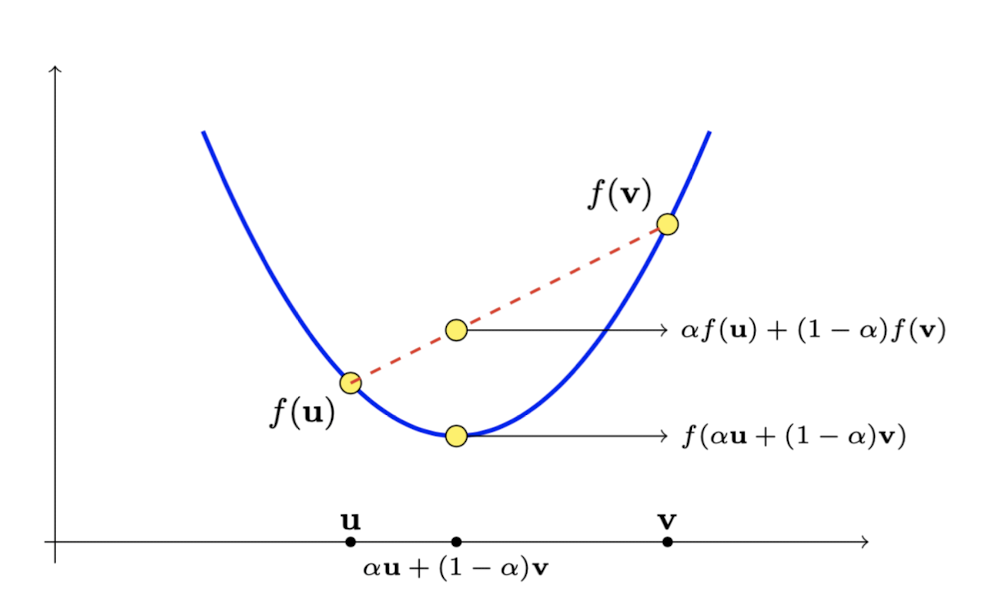
\includegraphics[width=0.7\linewidth]{pic1.png}
    % \caption{Caption}
    % \label{fig:enter-label}
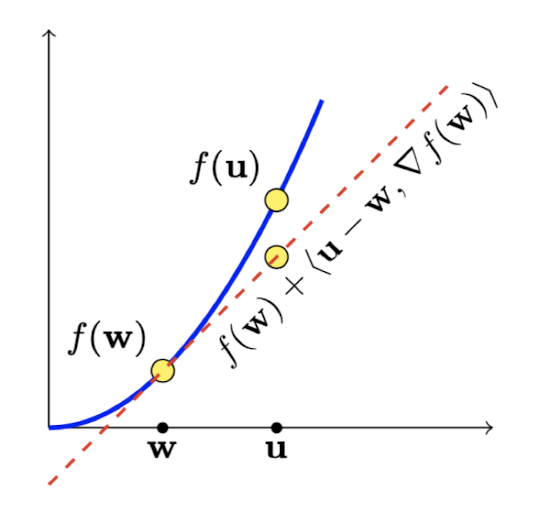
\includegraphics[width=0.5\linewidth]{pic2.png}
\end{minipage}}

\fbox{\begin{minipage}[t]{\linewidth}

\textbf{Properties of convex functions}
\begin{itemize}
    \item Every local minimum is also a global minimum
    \item For every $w$ the tangent at $(w)$ lies below $f$:
    \begin{itemize}
        \item $\forall u, f(u) \geq f(w) + \langle \nabla f(w), u - w \rangle$
    \end{itemize}
    \item If $f: \mathbb{R} \to \mathbb{R}$ is twice differentiable, then
    \begin{itemize}
        \item $f$ is convex
        \item $f'$ is monotone nondecreasing
        \item $f''$ is nonnegative
    \end{itemize}
    \item Are equivalent
\end{itemize}
    % 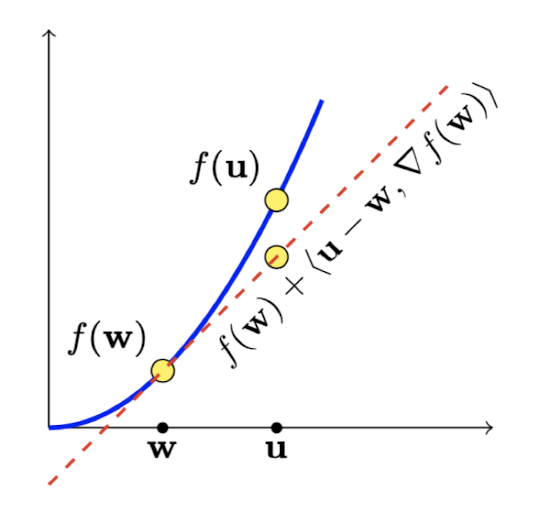
\includegraphics[width=0.5\linewidth]{pic2.png}

\end{minipage}}

\fbox{\begin{minipage}[t]{\linewidth}
\textbf{Combining convex functions}
\begin{itemize}
    \item If $g$ is convex, then $f(w) = g((w,x) + y)$ is convex
    \item If $f_i$ are convex functions
    \begin{itemize}
        \item $g(x) = \max_{i} f_i(x)$ is convex
        \item $g(x) = \sum w_i f_i(x)$ is convex
        \begin{itemize}
            \item Loss function convex, average of loss is also convex
        \end{itemize}
    \end{itemize}
\end{itemize}

\end{minipage}}

\fbox{\begin{minipage}[t]{\linewidth}
\textbf{Convex learning - Gradient}
\begin{itemize}
    \item Gradient (a vector derivative in multiple dimensions)
    \begin{itemize}
        \item The direction and speed of fastest increase
        \[ \nabla f(w) = \left( \frac{\partial f(w)}{\partial w_1}, \ldots, \frac{\partial f(w)}{\partial w_d} \right) \]
    \end{itemize}
    \item (here a $w_i$ is a parameter or dimension of the model)

\end{itemize}

\end{minipage}}

\fbox{\begin{minipage}[t]{\linewidth}

\textbf{Gradient descent}
\begin{itemize}
    \item Gradient is
    \[ \nabla f(w) = \left( \frac{\partial f(w)}{\partial w[1]}, \ldots, \frac{\partial f(w)}{\partial w[d]} \right) \]
    \item Gradient represents the direction in which $f$ increases fastest
    \item Gradient Descent: At every step $t$:
    \begin{itemize}
        \item $w^{t+1} = w^t - \eta \nabla f(w^t)$
        (Move in the direction that $f$ decreases fastest With a step scale of $\eta$)
    \end{itemize}
    \item After T steps, output the average vector
    $W = \frac{1}{T} \sum_{t=1}^{T} w^t $
    
    \textbf{why not optimal ones? - }

\end{itemize}
\end{minipage}}


\fbox{\begin{minipage}[t]{\linewidth}
\textbf{Lipschitzness} 
Let \( C \subset \mathbb{R}^d \). A function \( f : \mathbb{R}^d \to \mathbb{R}^k \) is \(\rho\)-Lipschitz over \( C \) if for every \( w_1, w_2 \in C \) we have that
$ \|f(w_1) - f(w_2)\| \leq \rho \|w_1 - w_2\|.$ \\

A $\rho$-Lipschitz function has bounded rate of change - the distance between outputs grows at most $\rho$ times faster than the distance between inputs. This implies: The function cannot change too rapidly, If differentiable, its gradient norm is bounded by $\rho$, Important for optimization stability
    
\end{minipage}}


\fbox{\begin{minipage}[t]{\linewidth}
\textbf{For convex lipschitz bounded learning} 
    \begin{itemize}
        \item Setting $\eta = \sqrt{\frac{B^2}{\rho^2 T}}$
        \item We can get
        $f(\bar{w}) - f(w^*) \leq \frac{B \rho}{\sqrt{T}} \quad$. (Increase T, decrease loss, fairly close to optimum loss)
        \item Alternatively, to achieve $f(\bar{w}) - f(w^*) \leq \epsilon $  the number of rounds is: $T \geq \frac{B^2 \rho^2}{\epsilon^2} $
    \end{itemize}

\end{minipage}}

\fbox{\begin{minipage}[t]{\linewidth}
\textbf{Stochastic Gradient Descent} 
\begin{itemize}
    \item Idea: Instead of computing gradient on the entire dataset each time, compute them on small samples: Small batches of data, Or even a single data point (Each i.i.d data point is treated like a tiny sample of data)
    \item While any single data point does not represent the set, on average they behave similarly
    \item GD vs SGD: SGD takes a more random path, but follows similar trends
\end{itemize}
\textbf{SGD for minimising f(w)}\\
parameters: Scalar $\eta > 0$, integer $T > 0$
\\ initialize: $w^{(1)} = 0$
\\ for $t = 1, 2, \ldots, T$ 
\begin{itemize}
    \item choose $v_t$ at random from a distribution such that $\mathbb{E}[v_t | w^{(t)}] \in \partial f(w^{(t)})$ 
    \item update $w^{(t+1)} = w^{(t)} - \eta v_t$
\end{itemize}
output $\bar{w} = \frac{1}{T} \sum_{t=1}^{T} w^{(t)}$

\textbf{Theorem (14.8)}
Similar result to deterministic GD:
    $\mathbb{E} \left[ f(\bar{\mathbf{w}}) \right] - f(\mathbf{w}^*) \leq \frac{B \rho}{\sqrt{T}} $
\end{minipage}}


\fbox{\begin{minipage}[t]{\linewidth}
\textbf{Modifications} 
\begin{itemize}
    \item For large neural nets
    \begin{itemize}
        \item Simply put all edge weights in the same vector
        \item SGD algorithm does not depend on what your model type is, as along as all parameters are real-valued
    \end{itemize}
    \item Mini batching:
    \begin{itemize}
        \item Instead of one data item at time, take them in batches of a few at a time.
        \item Faster, and fewer unhelpful moves
    \end{itemize}
    \item Run in epochs. In each epoch
    \begin{itemize}
        \item Order the data points in a random permutation
        \item For each data point (or mini-batch)
        \begin{itemize}
            \item Compute the gradient and move the modes
        \end{itemize}
    \end{itemize}
    \item Other modifications:
    \begin{itemize}
        \item Change learning rates
        \item Add momentum, add dropout etc
    \end{itemize}
\end{itemize}

\end{minipage}}



\fbox{\begin{minipage}[t]{\linewidth}
\textbf{Strong Convexity}
\begin{itemize}
    \item Function $f$ is $\lambda$-strongly convex if
    \[ f(\alpha w + (1 - \alpha)u) \leq \alpha f(w) + (1 - \alpha)f(u) - \frac{\lambda}{2} \alpha (1 - \alpha) \|w - u\|^2 \]
\end{itemize}

\end{minipage}}

\fbox{\begin{minipage}[t]{\linewidth}
\textbf{Smoothness}
$f$ is $\beta$-smooth if $\nabla f$ is $\beta$-Lipschitz:
 $||\nabla f(v) - \nabla f(w)|| \leq \beta ||v - w||$
\end{minipage}}

\fbox{\begin{minipage}[t]{\linewidth}
\textbf{Convex-Lipschitz-Bounded learning problems}
A learning problem $(H, Z, \ell)$ where:
\begin{itemize}
    \item $H$ is convex, $\forall w \in H$, $|w| \leq B$
    \item $\forall z \in Z$ the loss $l(\cdot, z)$ is convex and $\rho$-Lipschitz (for some $\rho$)
\end{itemize}
\end{minipage}}

\fbox{\begin{minipage}[t]{\linewidth}
\begin{itemize}
    \item Convex Hypothesis Class $\mathcal{H}$: The set of possible models forms a "bowl-shaped" space where any interpolation between two models is also valid, ensures optimization has no local minima—gradient descent can find the global optimum.
    \item Lipschitz Loss: The loss function’s output changes smoothly—small changes to the model weights $w$ don’t cause abrupt jumps in loss.
    \item The model weights are constrained to a "finite-sized" space
\end{itemize}
\end{minipage}}

\fbox{\begin{minipage}[t]{\linewidth}
\textbf{Convex-smooth-bounded learning}
A learning problem $(H, Z, \ell)$ where:
\begin{itemize}
    \item $H$ is convex, $\forall w \in H$, $||\boldsymbol{w}|| \leq B$
    \item $\forall z \in Z$ the loss $\ell(\cdot, z)$ is convex, nonnegative and $\beta$-smooth (for some $\beta$)
\end{itemize}

\end{minipage}}

\fbox{\begin{minipage}[t]{\linewidth}
\textbf{Why do we want convexity, smoothness, lipschitzness etc?}
\begin{itemize}
    \item Avoids sudden changes in function and its gradients
    \item Easier to compute and apply gradients as optimization steps
    \item Most theoretical analysis assume some of these properties
    \item Most practical situations have similar properties
    \begin{itemize}
        \item For most regions of data space and model space
        \item It is hard to make SGD, or any algorithm work if it does not
    \end{itemize}
    \end{itemize}
\end{minipage}}


\fbox{\begin{minipage}[t]{\linewidth}

\textbf{What is the problem of 0-1 empirical risk as loss function?}
Average empirical error as the loss - 
Not differentiable at that point,
derivative = 0 at other points, thus not useful
\end{minipage}}

\fbox{\begin{minipage}[t]{\linewidth}
\textbf{Surrogate loss functions}
\begin{itemize}
    \item Some loss functions are hard to work with: Not convex, hard to optimize for
    \item \textbf{Solution}
    \begin{itemize}
        \item "surrogate" loss function: Should be convex, should upper bound (be larger than original loss.)
    \end{itemize}
    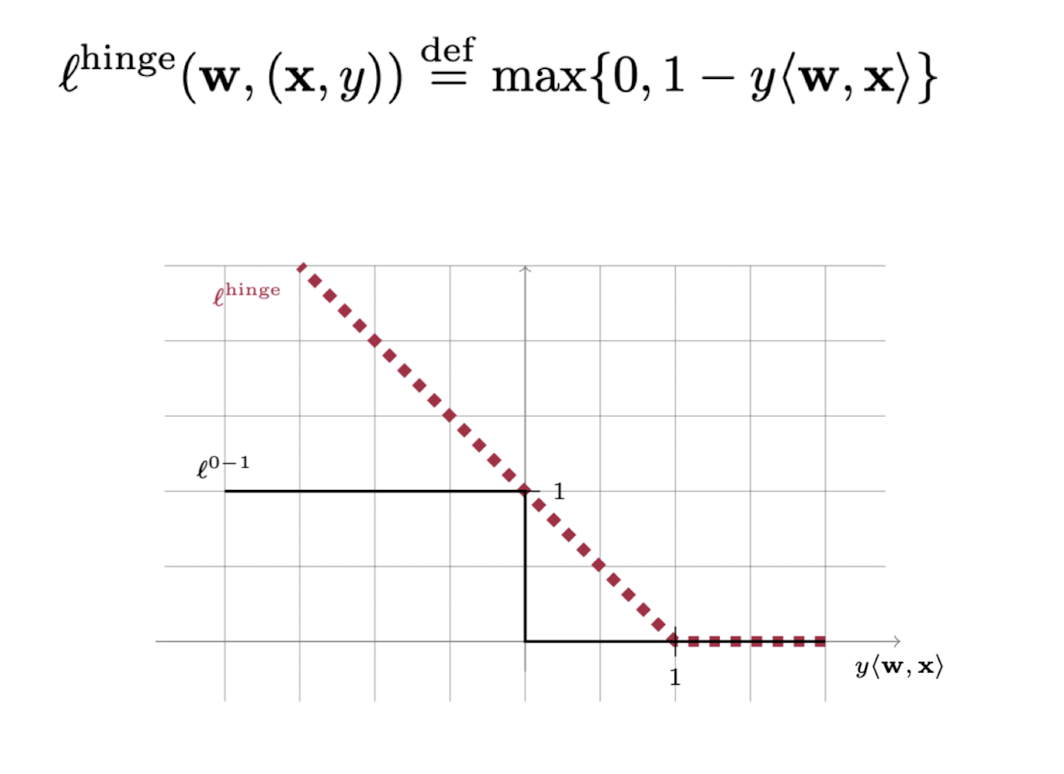
\includegraphics[width=0.9\linewidth]{pic3.png}
\end{itemize}
\end{minipage}}

\fbox{\begin{minipage}[t]{\linewidth}
\textbf{Regularization}
\begin{itemize}
    \item Min. loss with a regularization term:
     $\operatorname*{argmin}_{w} \left( L_S(w) + R(w) \right)$
    \item Commonly used: $R(w) = \lambda \| w \|^2$ (Called Tikhonov regularization)
\end{itemize}

\textbf{Smaller weights, less likely to overfit}\\
\textbf{Ridge regression}
\begin{itemize}
    \item Linear regression with Tikhonov regularization
    $\operatorname{argmin}_{\mathbf{w} \in \mathbb{R}^d} \left( \lambda \|\mathbf{w}\|_2^2 + \frac{1}{m} \sum_{i=1}^m \frac{1}{2} ( \langle \mathbf{w}, \mathbf{x}_i \rangle - y_i )^2 \right)$
\end{itemize}

\begin{itemize}
    \item $R(w) = \lambda \|w\|^2$ is 2$\lambda$-strongly convex
    \item If $f$ is $\lambda$-strongly convex and $g$ is convex, then $f + g$ is $\lambda$-strongly convex
    \item Thus, Ridge regression is strongly convex
    \item Strongly convex loss implies stability - useful property in SGD and other methods
\end{itemize}
\end{minipage}}

\fbox{\begin{minipage}[t]{\linewidth}
\textbf{Stability}
\begin{itemize}
    \item A learning algorithm is stable if: A small change to training set does not cause a big change to the output (model or hypothesis)
     \item It implies that it is not too sensitive to specific S. does not overfit
        \item If we continue to use it, it will not abruptly change behaviour
\end{itemize}

\begin{itemize}
    \item Suppose in $S$, we replace $z_i$ with $z' \sim D$
    \item Let us write this as $S^i$
    \item A good algorithm $A$ should have small value for $|\ell(A(S^i), z_i) - \ell(A(S), z_i)|$
    \item The loss on $z_i$ does not depend too much on it being in the sample
\end{itemize}
\end{minipage}}

\fbox{\begin{minipage}[t]{\linewidth}
\textbf{Stability definition and result}
\begin{itemize}
    \item Algorithm $A$ is on-average-replace-one-stable with rate $\epsilon(m)$
    \item If
    \[ \mathbb{E}\left[\ell(A(S^i), z_i) - \ell(A(S), z_i)\right] \leq \epsilon(m) \]
    \item Theorem: The generalization gap is bounded by the stability
    \[ \mathbb{E}[L_D(A(S)) - L_S(A(S))] = \mathbb{E}[\ell(A(S^i), z_i) - \ell(A(S), z_i)] \]
    
\end{itemize}
\end{minipage}}

\fbox{\begin{minipage}[t]{\linewidth}
\textbf{Generalisation Gap/Loss} \\
Empirical or training loss: $L_S(h)$ \\
Generalisation loss or true loss : $L_D(h)$ \\
$L_D(h) - L_S(h)$: A measure of overfitting

\end{minipage}}

\fbox{\begin{minipage}[t]{\linewidth}
\textbf{Uniform Stability}
\begin{itemize}
    \item Suppose we get $S^i$ by replacing one element $z_i$ at position $i$ of $S$ with a new element $z_i'$
    \item And suppose that $z \in Z$ is some possible input element
    \item As before, $A(S)$ refers to the model that algorithm $A$ computes using $S$
    \item We can write the loss on $z$ as $l(A(S),z)$
\end{itemize}
\end{minipage}}

\fbox{\begin{minipage}[t]{\linewidth}

\textbf{Algorithm $A$ is $\epsilon$-uniformly stable if}
\begin{itemize}
    \item \[ \text{Sup}_{z \in Z} [E_A l(A(S^i),z) - E_A l(A(S),z)] \leq \epsilon \]
    \item $E_A$ means expectation taken over all possible random behaviour of $A$
\end{itemize}
Replace 1 point, loss on other points should have similar expectations on all other points
\end{minipage}}

\fbox{\begin{minipage}[t]{\linewidth}
\textbf{Uniform Stability implies generalization}
    \begin{itemize}
        \item If Randomized Algorithm $A$ is $\epsilon$-uniformly stable then
        \[ E_S E_A \ell(A(S), D) \leq E_S E_A \ell(A(S), S) + \epsilon \]
        - True loss $\leq$ Training loss $+ \epsilon$
\end{itemize}
\end{minipage}}

\fbox{\begin{minipage}[t]{\linewidth}
\begin{itemize}
    \item Regularization creates strong convexity
    \item Strong convexity implies stability
    \item Stability implies generalization
\end{itemize}
\end{minipage}}


\fbox{\begin{minipage}[t]{\linewidth}
\textbf{Non-convexity}
Many minima in the space of models (edge weights) \\
\textbf{Neural Networks and Expressive Power}
\begin{itemize}
    \item \textbf{Step Activation}: Neurons with step activation can identify half-planes. Combining these allows creating arbitrary polygons for classification.
    \item \textbf{ReLU Activation}: 
    $f(x) = \max(0, x)$ \\
    ReLU splits the domain into cells and outputs a "score" representing distance from the boundary. Deep ReLU networks can exponentially increase the complexity of the function they compute.
    \item \textbf{Softmax}: Converts logits ($y_i$) into probabilities:
    \[ \text{softmax}(y_i) = \frac{e^{y_i}}{\sum_j e^{y_j}} \]
    \begin{itemize}
        \item Differentiable alternative to hard-max
        \item Normalized output can be interpreted as class probabilities
    \end{itemize}
\end{itemize}
\end{minipage}}


\fbox{\begin{minipage}[t]{\linewidth}
\textbf{Cross entropy loss}

\textbf{Loss Function and Generalisation}
\begin{itemize}
    \item \textbf{Cross Entropy Loss}: For true label vector $t$ and predicted probabilities $p$:
    $\ell_{CE} = -\sum t_i \ln p_i$
    \item \textbf{Generalisation Gap}: Difference between training and test loss. Overfitting occurs when the gap is large.
\end{itemize}

\end{minipage}}




\fbox{\begin{minipage}[t]{\linewidth}
\textbf{Overparameterised NN}
    \begin{itemize}
        \item High complexity and therefore high estimation error
        \item Expect heavy overfitting and high test/generalization loss/error
    \end{itemize}
    \textbf{Double Descent Phenomenon}:
    \begin{itemize}
        \item Traditional U-shaped test error curve
        \item Second descent when parameters exceed data points
        \item SGD finds solutions with good generalization despite overparameterization
    \end{itemize}

\end{minipage}}

\fbox{\begin{minipage}[t]{\linewidth}
\textbf{Weight Distribution}
\begin{itemize}
    \item \textbf{Post-Training Analysis}:
    \begin{itemize}
        \item Majority of weights cluster near zero
        \item Small fraction have significant magnitude
    \end{itemize}
    
    \item \textbf{Implications}:
    \begin{itemize}
        \item Effective dimensionality lower than parameter count
        \item Network capacity not fully utilized
    \end{itemize}
\end{itemize}
\end{minipage}}

\fbox{\begin{minipage}[t]{\linewidth}
\textbf{Network Pruning} Take all edges that are tiny weights and remove them.
Can sometimes remove 80\% - 90\% of edges, retains comparable performance and sometimes better generalization.\\
Standard pruning methods: One-shot: Train; Remove small weights; Return to initialisation weights and retrain; Stop\\
Iterative: Set random weights; Train; Remove edges with small weights; Start over
\end{minipage}}

\fbox{\begin{minipage}[t]{\linewidth}
\textbf{Lottery Ticket Hypothesis}:
    \begin{itemize}
        \item Randomly initialized dense network contains subnetworks that can give good performance.
        \item Algorithm:
        \begin{enumerate}
            \item Initialise a network to random weights
            \item Train for some iterations
            \item Prune p\% of edges with small weights
            \item Reset the remaining edges to their original random weights

        \end{enumerate}
        \item Matches performance of original network
    \end{itemize}
\end{minipage}}

\fbox{\begin{minipage}[t]{\linewidth}
\textbf{Pruning and Dimension}
\begin{itemize}
    \item The dimension of $\mathcal{H}$ is determined by the number of parameters
    \item The pruning and lottery tickets papers suggest that there are lower dimensional subspaces of H that contain good solutions
\end{itemize}
Start with a bigger subspace, allow optimisation algorithm to find the best suited one
\end{minipage}}

\fbox{\begin{minipage}[t]{\linewidth}
\textbf{Minimas} 

    \begin{itemize}
        \item Flat minima have small curvature in all directions - generalize better, more stable
        \item Sharp minima have large curvature in some directions - prone to overfitting: Take a slightly different model or slightly different data, loss will jump
    \end{itemize}
    
\end{minipage}}

\fbox{\begin{minipage}[t]{\linewidth}

\textbf{Quantifying Sharpness}
\begin{itemize}
    \item \textbf{$\epsilon$-Sharpness}: At min $\theta$ take ball $B(\theta, \epsilon)$ of radius $\epsilon$. Set of all points within a distance $\epsilon$ of $\theta$.
    \[ \max_{\theta' \in B(\theta,\epsilon)} \frac{L(\theta') - L(\theta)}{1 + L(\theta)} \]
    
    \item \textbf{Hessian Analysis (High dimension)}:

    \[
H_f =
\begin{pmatrix}
\frac{\partial^2 f}{\partial x_1^2} & \frac{\partial^2 f}{\partial x_1 \partial x_2} & \cdots & \frac{\partial^2 f}{\partial x_1 \partial x_n} \\
\frac{\partial^2 f}{\partial x_2 \partial x_1} & \frac{\partial^2 f}{\partial x_2^2} & \cdots & \frac{\partial^2 f}{\partial x_2 \partial x_n} \\
\vdots & \vdots & \ddots & \vdots \\
\frac{\partial^2 f}{\partial x_n \partial x_1} & \frac{\partial^2 f}{\partial x_n \partial x_2} & \cdots & \frac{\partial^2 f}{\partial x_n^2}
\end{pmatrix}
\quad \text{(size } n^2\text{)}
\]

    
    \[ loss = \begin{bmatrix}
    \frac{\partial^2 f}{\partial w_1^2} & \frac{\partial^2 f}{\partial w_1 \partial w_2} \\
    \frac{\partial^2 f}{\partial w_2 \partial w_1} & \frac{\partial^2 f}{\partial w_2^2}
    \end{bmatrix} \]
    \begin{itemize}
        \item Eigenvalues correspond to principal curvatures: Corresponding eigen vectors represent the directions of these curvatures
        \item Large eigenvalues indicate sharper minima
    \end{itemize}

\textbf{Algorithmic Approaches}:
    \begin{itemize}
        \item Sharpness-Aware Minimization (SAM): Use $\epsilon$ sharpness, Modifies the loss function:
        $L_{\text{SAM}}(\theta) = L(\theta) + \max_{\|\epsilon'\| \leq \epsilon} [L(\theta + \epsilon') - L(\theta)]$
        \item Entropy SGD: Optimizes a modified objective function, Computationally intensive due to additional complexity
        \item Stochastic Weight Averaging (SWA): Averages the weights of the last $c$ models during training, Empirical results show it produces flatter minima
    \end{itemize}
\end{itemize}
\end{minipage}}

\fbox{\begin{minipage}[t]{\linewidth}
\textbf{Flat Minima}

\begin{itemize}[leftmargin=1.5em]

    \item Sharp minima can sometimes perform well despite the preference for flat minima.
    \item Neural networks are highly redundant; many different weight configurations can represent the same function.
    \item It is possible to reconfigure weights such that the loss remains the same, but the curvature (sharpness) differs.
    
\end{itemize}
\textbf{SGD and Flat Minima}
\begin{itemize}[leftmargin=1.5em]
    \item Stochastic Gradient Descent (SGD) tends to favor flat, generalizable minima.
    \item Large batch sizes with small learning rates approximate smooth gradients and tend to find sharp minima.
    \item Small batch sizes with larger learning rates produce noisy updates that can escape sharp minima.
    \item SGD is likely to return to a flat minimum even after perturbations due to the size and stability of the flat region.
\end{itemize}
\end{minipage}}
%----------------------privacy-------------------------------------
\fbox{\begin{minipage}[t]{\linewidth}
\textbf{Differential Privacy Fundamentals}
Publish a noisy version of the true output:
$A(D) = f(D) + y$
where $y$ is random noise from a suitable distribution. 

\textbf{Formal Definition}
For neighbouring datasets $D$ and $D' = D \setminus \{x\}$, algorithm $A$ is $\epsilon$-differentially private if:
$\frac{1}{e^\epsilon} \leq \frac{\Pr[A(D) \in S]}{\Pr[A(D')\in S]} \leq e^\epsilon$

\end{minipage}}

\fbox{\begin{minipage}[t]{\linewidth}
\textbf{DP Key Properties}
\begin{itemize}
    \item Bounds the probability ratio of outputs for similar inputs
    \item $\epsilon$ controls privacy-accuracy tradeoff:
    \begin{itemize}
        \item Smaller $\epsilon$ = stronger privacy
        \item Larger $\epsilon$ = more accuracy
    \end{itemize}
\end{itemize}
\textbf{Computation-Centric Guarantee}
\begin{itemize}
    \item Protects whether data was used in computation
    \item Holds even if adversary knows: The algorithm, The noise distribution, All other data points
    \item Only unknown: The specific noise instantiation
\end{itemize}

\end{minipage}}

\fbox{\begin{minipage}[t]{\linewidth}
\textbf{Laplace Mechanism}
For function $f$ with $\ell_1$ sensitivity $\Delta f$:

\[
\mathcal{A}(D) = f(D) + \text{Lap}(\Delta f/\epsilon)
\]

Where the Laplace distribution has PDF:

\[
\text{Pr}[y] = \frac{1}{2b}e^{-|y|/b}, \quad b = \Delta f/\epsilon
\]
\end{minipage}}

\fbox{\begin{minipage}[t]{\linewidth}
\textbf{Private Counting Example}
\begin{itemize}
    \item True count: $n$
    \item Private release: $n + \text{Lap}(1/\epsilon)$
    \item Proof sketch for $\epsilon$-DP:
    \[
    \frac{\Pr[\text{noise}=y]}{\Pr[\text{noise}=y+1]} = e^{|y+1|\epsilon - |y|\epsilon} \leq e^{\epsilon}
    \]
\end{itemize}
\end{minipage}}

\fbox{\begin{minipage}[t]{\linewidth}
\begin{itemize}
    \item The noise distribution needs infinite support, therefore Laplace and Guassian where you need high concentration somewhere.
    \item Concentrated at zero: want noises to be small and stay close to original
\end{itemize}

\end{minipage}}

\fbox{\begin{minipage}[t]{\linewidth}
\textbf{Value vs. Presence Privacy}
\begin{itemize}
    \item \textbf{Removal DP}: Standard definition (hides presence)
    \item \textbf{Replacement DP}: Hides both presence and values
    \item Relationship: $2\epsilon$-DP for value changes

\end{itemize}
\end{minipage}}

\fbox{\begin{minipage}[t]{\linewidth}
\textbf{Group Privacy}
For group size $k$:
\begin{itemize}
    \item Standard $\epsilon$-DP becomes $k\epsilon$-DP
    \item Proof via ratio: $\frac{\Pr[y]}{\Pr[y+k]} = e^{k\epsilon}$
    \item Solution: Increase noise to $\text{Lap}(k/\epsilon)$ (Larger variance makes red ($n$) and blue ($n-k$) distribution more similar hence output similar probabilities) and attains $\epsilon-DP$
\end{itemize}

\end{minipage}}

\fbox{\begin{minipage}[t]{\linewidth}
\textbf{Sensitivity and Mechanisms} \\
\underline{Sensitivity Definition}: Sensitivity quantifies how much a single individual's data can maximally influence the output of a function $f$ when applied to a dataset.
\[
\Delta f = \max_{D,D'} |f(D) - f(D')|
\]

\underline{Laplace Mechanism}: To achieve differential privacy, we add noise scaled to the sensitivity.
\[
A(D) = f(D) + \text{Lap}(\Delta f/\epsilon)
\]
Smaller $\epsilon$ or larger $\Delta f$ increases error (privacy-utility tradeoff). 

\underline{Utility Guarantee}: Laplace method has an error bound. The error induced is determined by sensitivity, but not much larger. \\
Expected error: $\mathbb{E}[|A(D)-f(D)|] = \Delta f/\epsilon$

\end{minipage}}

\fbox{\begin{minipage}[t]{\linewidth}

\textbf{Variants of Differential Privacy}
\begin{enumerate}
    \item Local DP
        \begin{itemize}
        \item Each user adds noise locally: $X_i + \text{Lap}(1/\epsilon)$
        \item Protects individual data before collection
        \item Higher total noise than centralized approach
        \end{itemize}
    \item Approximate DP
        \begin{itemize}
            \item Algorithm A is $(\epsilon,\delta)$-differentially private if 
            \item For every neighbouring $D,D'$: \\ $\Pr[A(D) \in S] \leq e^\epsilon \Pr[A(D') \in S] + \delta$
            \item $\delta$ must be very small to be useful
            \item \textbf{Theorem: Gaussian Mechanism satisfies $(\epsilon,\delta)$-DP}
        \end{itemize}
        
        
\end{enumerate}


\end{minipage}}

\fbox{\begin{minipage}[t]{\linewidth}
\textbf{Gaussian Mechanism} \\
The probability density function of a Gaussian (normal) distribution is:
\[
N(\mu, \sigma^2) = \frac{1}{\sigma\sqrt{2\pi}} e^{\left( -\frac{(y-\mu)^2}{2\sigma^2} \right)}
\]
\begin{enumerate}
    \item Compute the function output $f(D)$ and its sensitivity $\Delta f$
    \item Generate noise from a zero-mean Gaussian:
    $y \sim N(0, \sigma^2),    \sigma = \frac{\sqrt{2\ln\left( \frac{1.25}{\delta} \right)} \Delta f}{\epsilon}$
    \item Output the noisy result: $f(D) + y$
\end{enumerate}
\end{minipage}}

\fbox{\begin{minipage}[t]{\linewidth}
\textbf{Composition}
For $k$ mechanisms with $(\epsilon_i,\delta_i)$-DP:
\[
\epsilon_{\text{total}} = \sum \epsilon_i, \quad \delta_{\text{total}} = \sum \delta_i
\]
$\epsilon, \delta$ increase, lose more privacy as more computations are released.\\
To get $\epsilon$-DP, each query add noise of $\frac{\epsilon}{k}$ \\
Differential privacy holds for further use of output $m$ obtained with an $\epsilon$-DP algorithm. \\


\textbf{Amplification by Sampling}
Given:
\begin{itemize}
    \item An algorithm $A$ that is $(\epsilon, \delta)$-differentially private for dataset $D$
    \item A sampling procedure $S(D)$ where each element appears with probability $p$
\end{itemize}

Then the composed algorithm $A(S(D))$ satisfies:
\[
(\epsilon', p\delta)\text{-differential privacy}
\]
where:
\[
\epsilon' = \ln\big(1 + p(e^{\epsilon} - 1)\big) \leq 2p\epsilon
\]

\textbf{Key Implications}
\begin{itemize}
    \item Privacy improves (lower $\epsilon'$) when using randomly sampled batches ($p < 1$)
    \item The $\delta$ parameter scales linearly with sampling probability
    \item Particularly useful for DP-SGD with mini-batches
\end{itemize}

\end{minipage}}

\fbox{\begin{minipage}[t]{\linewidth}
\begin{itemize}
    \item \textbf{Algorithmic Property}: DP is a characteristic of the randomized algorithm, not the dataset itself. 
    
    \item \textbf{Noise Determination}:
    \begin{itemize}
        \item Noise scales with \textit{sensitivity} ($\Delta f$)
        \item Sensitivity must be \textit{pre-defined} (not computed from data to avoid leaks)
        \item Noise is calculated for \textit{all possible inputs}, not tailored to specific data points
    \end{itemize}
    Therefore, DP is determined based on the assumptions about the data, but not on the actual data. 
\end{itemize}

\end{minipage}}


\fbox{\begin{minipage}[t]{\linewidth}
\textbf{Multi-Dimensional Outputs:} \\
\textbf{Sensitivity Norms}
\begin{itemize}
    \item $L_1$ sensitivity: $\Delta_1 f = \max \|f(D)-f(D')\|_1 =  \|x - y\|_1 = |x_1 - y_1| + |x_2 - y_2| + \cdots + |x_k - y_k|$ 
    \item $L_2$ sensitivity: $\Delta_2 f = \max \|f(D)-f(D')\|_2 =   \|x - y\|_2 = \sqrt{(x_1 - y_1)^2 + (x_2 - y_2)^2 + \cdots + (x_k - y_k)^2}$
\end{itemize}

\textbf{Vector Mechanisms}
\begin{itemize}
    \item Laplace: $y_i \sim \text{Lap}(\Delta_1 f/\epsilon)$
    \item In high-dim, L2 sensitivity is smaller. 
    \item Gaussian: $y_i \sim N(0, (\Delta_2 f \sqrt{2\ln(1.25/\delta)}/\epsilon)^2)$
\end{itemize}
\begin{itemize}
\item \textbf{Choose Laplace} when:
\begin{itemize}
\item You need pure DP ($\delta=0$)
\item Working with small-dimensional outputs
\end{itemize}
\item \textbf{Choose Gaussian} when:
\begin{itemize}
\item High-dimensional outputs (e.g., ML models)
\item Can tolerate small $\delta>0$
\item Want smaller noise magnitude in high dimensions
\end{itemize}
\item In high dimensions ($k \gg 1$), Gaussian is preferable because: L2 sensitivity ($\sqrt{k}$) grows much slower than L1 ($k$), Noise scales as $\sqrt{k}$ instead of $k$
\item Since sensitivity determines the standard deviation of distribution, gaussian mechanism has smaller standard deviation. 
\end{itemize}
\end{minipage}}


\fbox{\begin{minipage}[t]{\linewidth}
\textbf{Differentially Private ML}: Adding vector $Y$ with $n$ parameters of noise to $\mathbf{w}$ (output of training algorithm).
\begin{itemize}
    \item \textbf{Output Perturbation for ERM}

    \item \textbf{DP-SGD Algorithm}: Non-convex optimisation where you do not know where the minimum could be. Thus, a different method for SGD.
    Standard SGD gradients can leak individual data points.
\end{itemize}

\end{minipage}}


\fbox{\begin{minipage}[t]{\linewidth}

\textbf{From Regularized ERM to DP ERM}
\\ 
\textbf{Regularized ERM Framework}
The standard regularized empirical risk minimization problem is:
\[
\hat{w} = \operatorname*{argmin}_{w} \big( L_{S}(w) + \lambda\|w\|^2 \big)
\]
where:
\begin{itemize}
    \item $L_S(w)$ is the empirical loss over dataset $S$
    \item $\lambda\|w\|^2$ provides $2\lambda$-strong convexity
    \item $L$ is convex, differentiable, and $G$-Lipschitz
\end{itemize}

\textbf{Connecting to Differential Privacy (Theorem)}
The $L_2$-sensitivity of ERM solutions is fundamentally bounded by:
\[
\Delta_2 f \leq \frac{4G}{n\lambda}
\]
This key result enables differential privacy through output perturbation:
\end{minipage}}



\fbox{\begin{minipage}[t]{\linewidth}
\begin{itemize}
    \item \textbf{DP-ERM Mechanism}: 
    \[
    w_{\text{private}} = \hat{w} + Y, \quad Y \sim N\left(0, \sigma^2 I\right)
    \]
    where the noise variance scales with sensitivity:
    \[
    \sigma = \frac{4G\sqrt{2\ln(1.25/\delta)}}{n\lambda\epsilon}
    \]
    
    \item \textbf{Privacy Guarantee}: This construction satisfies $(\epsilon,\delta)$-DP because:
    \begin{itemize}
        \item Strong convexity controls how much individual data points can affect $\hat{w}$
        \item The Gaussian noise magnitude is precisely calibrated to the sensitivity bound
        \item The regularizer $\lambda$ appears in both the sensitivity bound and noise term
    \end{itemize}
\end{itemize}

\textbf{Key Insights}
\begin{itemize}
    \item Regularization does double duty:
    \begin{itemize}
        \item Prevents overfitting (standard ML benefit)
        \item Bounds sensitivity for privacy (DP benefit)
    \end{itemize}
    \item The privacy-accuracy tradeoff is controlled by:
    \[
    \text{Noise} \propto \frac{1}{\lambda\epsilon} \quad \text{vs.} \quad \text{Bias} \propto \lambda
    \]
    \item Larger $\lambda$ reduces sensitivity but increases estimation bias
\end{itemize}

\end{minipage}}

\fbox{\begin{minipage}[t]{\linewidth}
\textbf{DP-SGD}

\textbf{Key Modifications for Privacy}
\begin{enumerate}
    \item Sample a point of batch $z$
    \item Compute Gradient $g_t = \nabla f_{w_t}(z)$
    \item \textbf{Gradient Clipping}:
    \[
    \widehat{g_t} = g_t \cdot \left(1, \frac{1}{\max(1,\frac{\|g_t\|}{C})}\right)
    \]
    \begin{itemize}
        \item Bounds $L_2$ sensitivity per sample to $C$
        \item Limits influence (sensitivity) of any one point
    \end{itemize}
    \item \textbf{Gaussian Noise Injection}:
    \[
    \widehat{g_t} \leftarrow \widehat{g_t} + \mathcal{N}(0, \sigma^2 C^2 I)
    \]
    \begin{itemize}
        \item Noise scaled to clipping bound $C$
        \item $\sigma$ depends on privacy budget $(\epsilon,\delta)$
    \end{itemize}
    \item Update model $w_{t+1} = w_t - \eta g_t$
\end{enumerate}
\end{minipage}}



\fbox{\begin{minipage}[t]{\linewidth}
\textbf{Privacy Analysis of DP-SGD}
\begin{itemize}
    \item \textbf{Per-step Guarantee}: Impact of data point(s) used in any one step is limited to a vector of length $C$.
    \[
    \sigma = \frac{\sqrt{2\ln(1.25/\delta)}}{\epsilon} \Rightarrow (\epsilon,\delta)\text{-DP per step}
    \]
    
    \item \textbf{Composition}:
    \begin{itemize}
        \item Basic: $(qT\epsilon, qT\delta)$-DP for $T$ steps, $q$ fraction of data 
        \item Tighter: $(q\epsilon\sqrt{T}, \delta)$-DP using advanced composition
    \end{itemize}
    
    \item \textbf{Amplification by Sampling}:
    \begin{itemize}
        \item Batches of size $q$ provide $\approx q\epsilon$ privacy cost
    \end{itemize}
\end{itemize}

\textbf{Why These Modifications?}
\begin{itemize}
    \item Clipping controls sensitivity (necessary for DP)
    \item Gaussian noise hides individual contributions
    \item Composition theorems account for multiple exposures
    \item Sampling amplification reduces privacy cost
\end{itemize}

\end{minipage}}

\fbox{\begin{minipage}[t]{\linewidth}
\textbf{Non-Numerical Queries and the Exponential Mechanism}

\textbf{Challenge with Non-Numerical Outputs} \\
Standard DP mechanisms (Laplace/Gaussian) require real-valued outputs. For discrete outputs:
\begin{multline*}
f: \mathcal{D} \to \mathcal{O} \quad \\ \text{where $\mathcal{O}$ is finite (e.g., \{movie\_titles, dates, categories\})}    
\end{multline*}


\begin{itemize}
    \item A \textbf{scoring function} $s: \mathcal{Z}^n \times \mathcal{O} \to \mathbb{R}$ 
    \item \textbf{Sensitivity} 
    \[\Delta s = \max_{o \in \mathcal{O}} \max_{D, D'} |s(D,o) - s(D',o)|\] - largest difference among all neighbouring dataset
\end{itemize}
\end{minipage}}

\fbox{\begin{minipage}[t]{\linewidth}
\textbf{Exponential Mechanism Solution}
Given a task to find $f(D)$:
\begin{itemize}
    \item Compute the scoring function $s(D,o)$ and its sensitivity $\Delta s$
    
    \item Output $o \in \mathcal{O}$ with probability:
    \[
    \Pr[o] = \frac{e^{\frac{\epsilon s(D,o)}{2\Delta s}}}{\sum\limits_{o' \in \mathcal{O}} e^{\frac{\epsilon s(D,o')}{2\Delta s}}}
    \]
    where:
    \begin{itemize}
        \item Higher privacy ($\epsilon \to 0$) reduces score differences
        \item Denominator provides normalization
    \end{itemize}
    
    \item Sampling properties:
    \begin{itemize}
        \item Probability decays exponentially with decreasing score
        \item High-scoring outputs are exponentially more likely
    \end{itemize}
    \item Relationship to Laplace:
    \begin{itemize}
        \item Generalizes Laplace mechanism to non-numeric outputs
        \item When $\mathcal{O} \subset \mathbb{R}$ and $s(D,o) = -|f(D)-o|$, recovers Laplace noise addition
    \end{itemize}
\end{itemize}
\end{minipage}}

\fbox{\begin{minipage}[t]{\linewidth}
\textbf{Key Properties of Exponential Mechanism}
\begin{itemize}
    \item Satisfies $\epsilon$-DP for any arbitrary output space $\mathcal{O}$
    \item Favours high-utility outputs ($s(D,o)$) exponentially
    \item Generalizes Laplace mechanism (when $\mathcal{O} \subset \mathbb{R}$ and $s(D,o) = -|f(D) - o|$)
\end{itemize}

\end{minipage}}
% Fairness---------------------------------------------------
\fbox{\begin{minipage}[t]{\linewidth}
\textbf{Key Fairness Definitions} -
\textbf{Individual Fairness}: Two people with similar features are treated similarly.  \\
Given:
\begin{itemize}
    \item Data points $V$
    \item Classes $C = \{0,1\}$
    \item Randomized classifier $f: V \to \Delta C$ where $\Delta C$ is the set of probability distributions over $C$
\end{itemize}

\noindent Example classifier output:
$
f(x) = (0.2, 0.8) \quad \text{(20\% class 0, 80\% class 1)}
$

\textbf{Fairness Condition}
A classifier $f$ is \textit{individually fair} if:
\[
\forall x, y \in V, \quad D(f(x), f(y)) \leq d(x, y)
\]
where:
\begin{itemize}
    \item $d: V \times V \to [0,1]$ measures distance between inputs
    \item $D: \Delta C \times \Delta C \to \mathbb{R}$ measures distance between output distributions
\end{itemize}
A useful individually fair classifier must be randomized

\end{minipage}}

\fbox{\begin{minipage}[t]{\linewidth}
\textbf{Utility Considerations in Fair Classification}
\\
\textbf{Limitations of Fairness Constraints}
\begin{itemize}
    \item Constant classifiers (e.g., $f(x) = (0.5, 0.5)$) satisfy:
    \[
    \forall x, y \in V, \quad D(f(x), f(y)) \leq d(x, y)
    \]
    but provide no useful discrimination
    
    \item Fairness condition alone is insufficient - must also consider predictive utility
\end{itemize}

\textbf{Utility Maximization}
The optimal fair classifier should:
\begin{itemize}
    \item Minimize the deviation from true labels:
    \[
    L(f, V) = \frac{1}{|V|} \sum_{x \in V} \big|\mathbb{E}[f(x)] - t(x)\big|
    \]
    where $t(x)$ is the true class label for $x$
    \end{itemize}

\textbf{Key Observations}
\begin{itemize}
    \item \textbf{Fairness Guarantees}:
    \begin{itemize}
        \item Apply to the \textit{probability distribution} of classifications
        \item Individual classifications may still appear unfair due to randomness
    \end{itemize}
    
    \item \textbf{Group Considerations}:
    \begin{itemize}
        \item Individual fairness does not ensure group fairness
        \item May perpetuate biases if groups have systematically different features
    \end{itemize}
\end{itemize}
\end{minipage}}

\fbox{\begin{minipage}[t]{\linewidth}

\textbf{Group Fairness}
\begin{itemize}
    \item \textbf{Demographic Parity}: A classifier C satisfies demographic parity if C is independent of sensitive attribute A. (Reverse DI)
    \[
    \Pr_{a}\{C=1\} = \Pr_{b}\{C=1\}
    \]
    
    \item \textbf{Equalized Odds/Positive Rate Parity (PRP)}:
    \begin{itemize}
        \item  True positive parity (TPP): $ \Pr_a\{C=1|Y=1\} = \Pr_b\{C=1|Y=1\}$
        \item False Positive Parity (FPP): $\Pr_a\{C=1|Y=0\} = \Pr_b\{C=1|Y=0\}$
    \end{itemize}
   
    \item \textbf{Predictive Value Parity (PVP)}:
    \begin{itemize}
        \item Positive Predictive Value Parity: $\Pr_a\{Y=1|C=1\} = \Pr_b\{Y=1|C=1\}$
        \item Negative Predictive Value Parity: $\Pr_a\{Y=1|C=0\} = \Pr_b\{Y=1|C=0\}$
        \item Classifier C satisfies PPV if it satisfies both above.
    \end{itemize}

\end{itemize}

\textbf{Impossibility Results}
\begin{itemize}
    \item \textbf{Kleinberg's Impossibility}:
    \begin{itemize}
        \item Calibration
        \item Balance for positive class
        \item Balance for negative class
    \end{itemize}
    Cannot be simultaneously satisfied except in trivial cases
    
    \item \textbf{PRP vs PVP}:
    \begin{itemize}
        \item With different base rates, must violate either:
        \item Positive rate parity or
        \item Predictive value parity
    \end{itemize}
\end{itemize}
\end{minipage}}

\fbox{\begin{minipage}[t]{\linewidth}
\textbf{Disparate Impact (Measure Group Unfairness)} 

For protected attribute $X$ ($X=0$ means protected), $Y$ is all other features and classifier $f$: Classifier $f$ has disparate impact $\tau (0 <\tau<1)$ if:
\[
DI = \frac{\Pr[f(Y)=1|X=0]}{\Pr[f(Y)=1|X=1]} \leq \tau \quad (\text{typically } \tau=0.8)
\]
If the protected class is positively classified less than $\tau$ times as often as the unprotected class.
\begin{itemize}
    \item Suitable if protected/unprotected status are uncorrelated to true value or qualification
    \item But data may be biased, thus look at DI
\end{itemize}
\textbf{Certification}: How to verify that classification based on $Y$ will not lead to DI?
\textbf{Any classifier $C$ will not have disparate impact if $X$ cannot be predicted from $Y$}
\begin{itemize}
    
    \item Suppose $g:Y \rightarrow X$ predicts protected group status, measure predictability of $X$ from $Y$:
    \begin{multline*}
         BER(g(Y), X) = \\\frac{\Pr(g(Y)=0|X=1)+\Pr(g(Y)=1|X=0)}{2}
    \end{multline*}

    \item Dataset is $\epsilon$-predictable if $\exists g:Y \rightarrow X$ with $BER \leq \epsilon$

\end{itemize}
\end{minipage}}

\fbox{\begin{minipage}[t]{\linewidth}
\textbf{Disparate Impact Characterization}
\begin{itemize}
    \item Let $B = \Pr[f(Y)=1|X=0]$ be the fraction of protected group ($X=0$) classified as $C=1$
    \item \textbf{Theorem} $D$ is $( \frac{1}{2} - \frac{B}{8} )$-predictable if and only if it admits a classifier with DI$=0.8$ 
\end{itemize}

\textbf{Proof Sketch}
\begin{itemize}
    \item \textbf{Forward Direction}:
    \begin{itemize}
        \item Given classifier $f$ with $DI=0.8$, construct predictor:
        \[
        g(Y) = \begin{cases}
        1 & \text{if } f(Y)=1 \text{ (predict unprotected)} \\
        0 & \text{if } f(Y)=0 \text{ (predict protected)}
        \end{cases}
        \]
        \item Compute Balanced Error Rate (BER): \\
        $BER(g) = \frac{1}{2}\left(\Pr[f=0|X=1] + \Pr[f=1|X=0]\right) \leq \frac{1}{2} - \frac{B}{8}$
    \end{itemize}
    
    \item \textbf{Reverse Direction}:
    \begin{itemize}
        \item Any predictor $g$ with BER $\leq \frac{1}{2}-\frac{B}{8}$ can be converted to a classifier meeting DI=0.8 \\
        $DI(g(Y), C) = \frac{\Pr(g(Y) = 1 | X = 0)}{\Pr(g(Y) = 1 | X = 1)} = \frac{B}{B + 1 - 2 \cdot BER(g(Y), X)} \leq \frac{B}{\frac{5B}{4}} = 0.8$
        \item Shows inherent tension between predictability and fairness
    \end{itemize}
\end{itemize}

\textbf{Key Implications}
\begin{itemize}
    \item \textbf{Fairness-Predictability Tradeoff}: Lower predictability enables better DI
    \item \textbf{Legal Threshold}: The 0.8 DI ratio corresponds to $\frac{1}{2}-\frac{B}{8}$ predictability bound
    \item \textbf{Testing Methodology}: To certify DI compliance, check if protected attribute $X$ can be predicted from $Y$ with BER $\leq \frac{1}{2}-\frac{B}{8}$
\end{itemize}

\end{minipage}}



\fbox{\begin{minipage}[t]{\linewidth}
\textbf{Removing DI}: Want a modified $(X,Y)$ so that $BER(g(Y),X) > \epsilon$ \\
\underline{Algorithm Steps}
\begin{enumerate}
    \item Define $p_y^x$ as the fraction of people with protected status $x$ having score $\leq y$
    
    \item For each data point $(x_i, y_i)$:
    \begin{itemize}
        \item Calculate percentile $p_{y_i}^{x_i}$ within its protected group: Where someone ranks within their own group
        
    \end{itemize}
    
    \item Find $y_i^{-1}$ in the non-protected group where:
    \[
    p_{y_i^{-1}}^{1-x_i} = p_{y_i}^{x_i}
    \]
    ($p_{y_i^{-1}}^{1-x_i}$ is the percentile rank that person i would have in opposite group. Then, find the score in the opposite group that lands at the same percentile)
    
    \item Repair the feature value:
    \[
    \bar{y}_i = \text{median}(y_i, y_i^{-1})
    \]
    For each individual, replace score with median of original score and the matched score from opposite score.
\end{enumerate}
\end{minipage}}

\fbox{\begin{minipage}[t]{\linewidth}
\textbf{Key Properties}
\begin{itemize}
    \item Preserves within-group rankings
    \item Equalizes distributions across protected groups
    \item For multiple features: apply separately to each
\end{itemize}

\textbf{Limitations}
\begin{itemize}
    \item May prevent perfect classification
    \item Permits trivial unfair classifiers that technically satisfy DI
    \item Assumption: Groups have equal intrinsic qualification distributions
    \begin{itemize}
        \item Often violated in real-world biased data
    \end{itemize}
\end{itemize}
\end{minipage}}

% \fbox{\begin{minipage}[t]{\linewidth}

% \end{minipage}}


\end{multicols*}

\end{document}